	\section{Цель работы}
		Разработать экспертную систему с использованием среды GURU.
		
	\section{Предметная область}
		Целевая ЭС выполняет функцию оценки платформ для социальной торговли. Социальная торговля -- онлайн-трейдинг на финансовых рынках в рамках социальной платформы, внутри которой трейдеры взаимодействуют друг с другом.
		
		На рисунке \ref{tree} изображено дерево целей экспертной системы. Дугами отмечены вершины И, отсутствием дуг ИЛИ.
		
		\begin{figure}[ht] 
			\center
			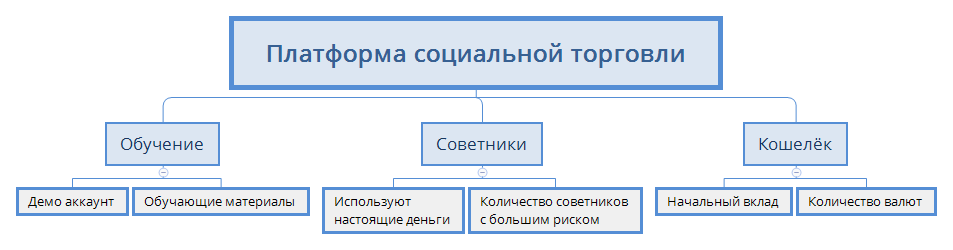
\includegraphics [width=\textwidth] {social-trading}
			\caption{Дерево целей} 
			\label{tree}
		\end{figure}
		\FloatBarrier
		
	\section{Описание ЭС}
	
	На основе дерева целей описаны переменные и правила, представленные в листинге.
	
	Системная переменная $ E.CFVA $, которая определяет формулу объединения факторов уверенности левой и правой частей правила имеет значение <<pp>>, т.е. фактор уверенности для операции <<И>> вычисляется по формуле $(a * b) / 100$, а для правила <<ИЛИ>> - по формуле 	$a + b - (a * b) / 100$
	
	Системная переменная $E.TRAC = <n>$ определяет режим работы системы – без трассировки.
	
	С помощью переменной $E.RIGR$ определяется режим проверки конфликтующих правил для достижения результата с заданной степенью точности. $E.RIGR = <с>$ – все возможные правила (полный перебор).
	
	Режим оценки $E.TRYP = <s>$ - проверка неизвестных переменных, пока значение какой-либо из них не будет получено.
	 
	$E.LNUM = 3$ -  длина числового значения для округления.
	
	$E.DECI = 0$ - число значащих цифр после запятой.
	
		
	\section{Листинг}
	
%	\lstinputlisting[caption={Листинг программы}]{listings/st.rss}
	
	\newpage
	\section{Примеры выполнения}
%		\begin{figure}[ht] 
%			\center
%			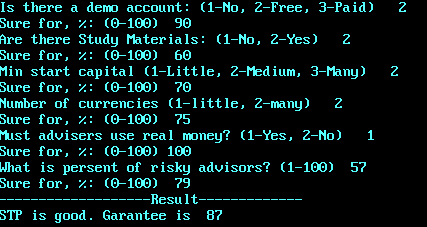
\includegraphics [width=\textwidth] {success}
%			\caption{Пример хорошей платформы} 
%		\end{figure}
%		\FloatBarrier
%		
%		\begin{figure}[ht] 
%			\center
%			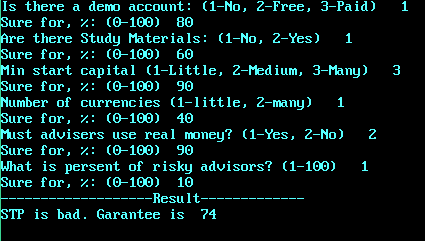
\includegraphics [width=\textwidth] {failure}
%			\caption{Пример плохой платформы} 
%		\end{figure}
%		\FloatBarrier
	
	\section{Вывод}
		В результате данной работы была спроектирована разработана ЭС, которая позволяет дать экспертную оценку платформам социальной торговли по введенным параметрам. Изучена программа GURU.